\documentclass{article}

\usepackage[polish]{babel}
\usepackage[utf8]{inputenc}
\usepackage[T1]{fontenc}
\usepackage{graphicx}
\usepackage{float}
\usepackage{listings}
\usepackage{color}
\usepackage[colorlinks=true]{hyperref}

\begin{document}
\renewcommand*{\tablename}{Tabela}
\begin{center}
{\huge \textsc{Zastosowania informatyki w logistyce}}

\vspace{0.8cm}
{\Large Tartak}
\vspace{0.8cm}

Krzysztof Skoracki
\vspace{0.5cm}

28 stycznia 2014
\vspace{1cm}
\end{center}

\section{Wprowadzenie}

Przedmiotem zadania jest tartak, działający w następujący sposób:

\begin{enumerate}
	\item{Drewno z magazynu wejściowego trafia do korowania}
	\item{Okorowane drewno zostaje pocięte na belki}
	\item{Belki trafiają albo do magazynu wyjściowego, albo zostają pocięte na deski}
\end{enumerate}

Pomiędzy stanowiskami oraz magazynami kursują wózki, które jednorazowo przewożą po jednej sztuce drewna.
Czas transportu drewna przez wózek wynosi 10\% czasu jego przetwarzania.
Różne rodzaje drewna charakteryzują się różnym czasem przetwarzania na poszczególnych maszynach.
Drewno podawane jest z magazynu wejściowego z użyciem algorytmu FIFO.

\section{Stan obecny}

\subsection{Finanse}

Roczny obrót wynosi 12 000 000zł.
Roczne koszty wynoszą 11 900 000zł.

Koszty dzielą się następująco:

\begin{itemize}
	\item{50\% --- koszty materiałowe}
	\item{50\% --- koszty pracownicze}
\end{itemize}

\subsection{Pracownicy}

Firma zatrudnia obecnie 50 pracowników:

\begin{itemize}
	\item{10 pracowników --- administracja}
	\item{10 pracowników --- wózki (5 wózków po 2 pracowników)}
	\item{30 pracowników --- maszyny}
\end{itemize}

Średni roczny koszt pracownika wynosi 119 000zł.

\subsection{Maszyny}

Typy, liczbę oraz wykorzystanie maszyn używanych w tartaku podano w tabeli \ref{table:mch}.

\begin{table}[H]
\center
\begin{tabular}{ c | c | c }
  \textbf{Typ} & \textbf{Liczba} & \textbf{Wykorzystanie} \\ \hline
  Korowanie & 3 & 50\% \\
  Belki & 1 & 50\% \\
  Deski & 2 & 50\% \\
\end{tabular}
\caption{Maszyny}
\label{table:mch}
\end{table}

\section{Optymalizacja}

\subsection{Założenia}
W ramach optymalizacji produkcji zastosowano szeregowanie zadań, które muszą być wykonane danego dnia.
Obecny algorytm FIFO zastąpiono uszeregowanie dającym najkrótszy czas przetwarzania.

W celu uszeregowania zadań użyto programu Lekin \footnote{\url{http://community.stern.nyu.edu/om/software/lekin/}}.

Dane wejściowe dla programu zostały wygenerowane losowo za pomocą przygotowanego skryptu.

Przykładowy zrzut ekranu z programu przedstawia rysunek \ref{fig:screen}.

\begin{figure}[H]
  \centering
  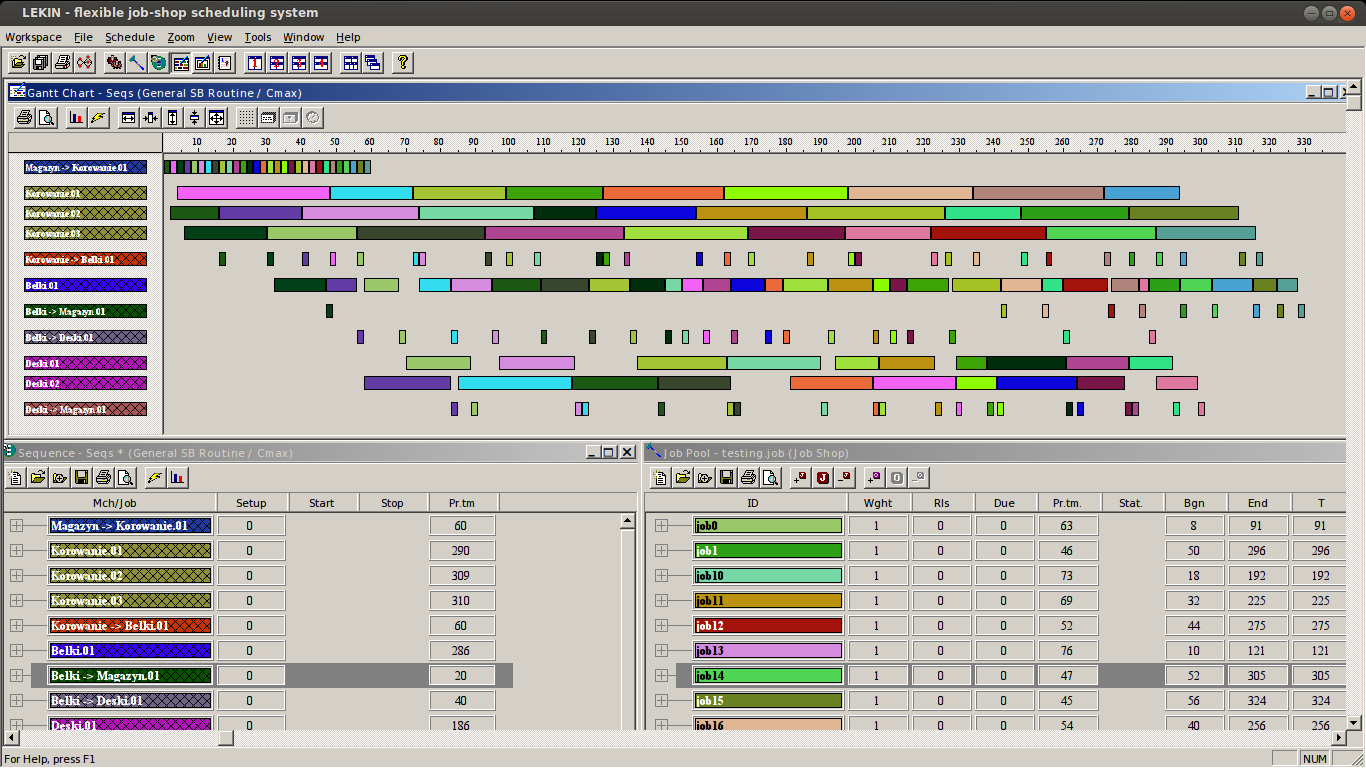
\includegraphics[width=12cm]{screenshot.png}
  \caption{Przykładowy zrzut ekranu z programu Lekin.}
  \label{fig:screen}
\end{figure}


\subsection{Wyniki}

W wyniku optymalizacji uzyskano wykorzystanie maszyn na poziomie około 80\%, w porównaniu do 50\% przed optymalizacją.

Zestawienie wyników finansowych przedstawiono w tabeli \ref{table:opt}.

\begin{table}[H]
\center
\begin{tabular}{ c | c | c }
   & \textbf{Przed optymalizacją} & \textbf{Po optymalizacji} \\ \hline
  Roczne koszty pracownicze (zł) & 5 950 000 & 5 950 000 \\
  Roczne koszty materiałowe (zł) & 5 950 000 & 9 520 000 \\
  Roczny przychód (zł) & 12 000 000 & 19 200 000 \\
  Roczny zysk (zł) & 100 000 & 3 730 000 \\
\end{tabular}
\caption{Wyniki optymalizacji}
\label{table:opt}
\end{table}

\section{Wnioski}

Ja widać, otrzymane wyniki finansowe przedstawiają się optymistycznie.
Trzeba jednak mieć na uwadze kilka kwestii:

\begin{enumerate}
	\item{Algorytm szeregujący zadania zakłada istnienie buforów przy każdym stanowisku pracy.
	Nie jest to do końca zgodne z założeniami zadania, natomiast analiza uszeregowania pokazuje, że brak buforów nie powinien mieć drastycznego wpływu na uzyskany poziom wykorzystania maszyn.}
	\item{Zatrudnienie osoby zarządzającej tartakiem najprawdopodobniej będzie kosztować więcej niż założone 50 000zł rocznie --- średnie koszty przypadające na pracownika są obecnie dużo wyższe.}
	\item{Zastosowanie wprowadzonego algorytmu szeregowania zadań wymaga odpowiedniego przeszkolenia pracownika obsługującego magazyn wejściowy.}
	\item{Nie brano pod uwagę nieliniowego wzrostu kosztów eksploatacji maszyn związanego ze zwiększeniem stopnia ich wykorzystania.}
\end{enumerate}

Mimo uwag zamieszczonych powyżej, zakup tartaku przy założeniu wprowadzenia opisanych usprawnień wydaje się opłacalną inwestycją.

\end{document}
